\documentclass{article}
% Encoding and language
\usepackage[T1]{fontenc}
\usepackage[utf8]{inputenc}
\usepackage{lmodern}
\usepackage[british]{babel}
% Page layout
\usepackage{lastpage}
\usepackage{geometry}
\geometry{margin=3cm}
\usepackage{parskip}
% Math
\usepackage{amsmath}
\usepackage{amssymb}
% Snippets for other math packages: ppla, pali, pbigi
% Visuals and code
\usepackage{graphicx}
\graphicspath{{pics/}}
\usepackage[labelformat=simple]{subcaption}
\renewcommand\thesubfigure{(\alph{subfigure})}
\usepackage{enumerate}
\usepackage{fancyvrb}
\usepackage{comment}
\usepackage{listingsutf8}
\usepackage{color}
\usepackage{parskip}


% LaTeX math commands

% Units
\newcommand{\uni}[1]{\ \mathrm{#1}}

\newcommand{\sciuni}[2]{\cdot10^{#1} \ \mathrm{#2}}

\newcommand{\dgr}{^{\circ}}

% Symbols, variables and operators
\newcommand{\ham}{\mathcal{H}}
\newcommand{\lag}{\mathcal{L}}


% Hyperbolic functions (only sech and csch as the others are defined by default)
\DeclareMathOperator{\sech}{sech}
\DeclareMathOperator{\csch}{csch}

% Inverse hyperbolic functions
\DeclareMathOperator{\arsinh}{arsinh}
\DeclareMathOperator{\arcosh}{arcosh}
\DeclareMathOperator{\artanh}{artanh}
\DeclareMathOperator{\arsech}{arsech}
\DeclareMathOperator{\arcsch}{arcsch}
\DeclareMathOperator{\arcoth}{arcoth}

% Inverse trigonometric functions (only arcsec, arccsc and arccot as the others are defined by default)
\DeclareMathOperator{\arcsec}{arcsec}
\DeclareMathOperator{\arcsc}{arccsc}
\DeclareMathOperator{\arccot}{arccot}

% Functions
\DeclareMathOperator{\erf}{erf}

% Complex analysis
\DeclareMathOperator*{\res}{Res}

\DeclareMathOperator{\wind}{wind}

\DeclareMathOperator{\re}{Re}

\DeclareMathOperator{\im}{Im}

\DeclareMathOperator{\Arg}{Arg}

\DeclareMathOperator{\Ln}{Ln}

\DeclareMathOperator{\pv}{P.V.}

% Linear algebra

% Defined by default: det, dim, ker

\DeclareMathOperator{\tr}{tr}

\DeclareMathOperator{\rank}{rank}

\newcommand{\inprod}[2]{\langle#1,#2\rangle}

% ------------------------------------------

\newcommand{\bra}[1]{\big\langle#1\big\rvert}
\newcommand{\Bra}[1]{\Big\langle#1\Big\rvert}
\newcommand{\sbra}[1]{\langle#1\rvert}

% ------------------------------------------

\newcommand{\ket}[1]{\big\lvert#1\big\rangle}
\newcommand{\Ket}[1]{\Big\lvert#1\Big\rangle}
\newcommand{\sket}[1]{\lvert#1\rangle}

% ------------------------------------------

\newcommand{\braket}[2]{\big\langle#1\big\lvert#2\big\rangle}
\newcommand{\Braket}[2]{\Big\langle#1\Big\lvert#2\Big\rangle}

% ------------------------------------------

\newcommand{\ketbra}[2]{\big\lvert#1\big\rangle\big\langle#2\big\rvert}
\newcommand{\Ketbra}[2]{\Big\lvert#1\Big\rangle\Big\langle#2\Big\rvert}

% ------------------------------------------

\newcommand{\exval}[1]{\big\langle#1\big\rangle}
\newcommand{\Exval}[1]{\Big\langle#1\Big\rangle}

% ------------------------------------------

\newcommand{\exvstate}[2]{\big\langle#2\big\lvert#1\big\rvert#2\big\rangle}
\newcommand{\Exvstate}[2]{\Big\langle#2\Big\lvert#1\Big\rvert#2\Big\rangle}

% ------------------------------------------

\newcommand{\matel}[3]{\big\langle#1\big\lvert#2\big\rvert#3\big\rangle}
\newcommand{\Matel}[3]{\Big\langle#1\Big\lvert#2\Big\rvert#3\Big\rangle}

% ------------------------------------------

\newcommand{\comm}[2]{\big[#1, #2\big]}
\newcommand{\Comm}[2]{\Big[#1, #2\Big]}

% ------------------------------------------

\newcommand{\acomm}[2]{\big\{#1, #2\big\}}
\newcommand{\Acomm}[2]{\Big\{#1, #2\Big\}}

% Vectors

\newcommand{\unitv}[1]{\mathbf{\hat{#1}}}

\newcommand{\unitg}[1]{\boldsymbol{\hat{#1}}}

\newcommand{\vtr}[1]{\mathbf{#1}}

\newcommand{\vtg}[1]{\boldsymbol{#1}}


% Calculus

\newcommand{\eval}[3]{\left[#1\right]_{#2}^{#3}}

\newcommand{\Eval}[3]{\Big[#1\Big]_{#2}^{#3}}

\newcommand{\partc}[3]{\left(\pdv{#1}{#2}\right)_{#3}}

\newcommand{\totdf}[3]{\left(\pdv{#1}{#2}\right)_{#3}\odif{#2} + \left(\pdv{#1}{#3}\right)_{#2}\odif{#3}}

\newcommand{\ft}[2]{\mathcal{F}[#1](#2)}

\newcommand{\ift}[2]{\mathcal{F}^{-1}[#1](#2)}

\newcommand{\lt}[2]{\mathcal{L}[#1](#2)}

\newcommand{\ilt}[2]{\mathcal{L}^{-1}[#1](#2)}

% Sets

\newcommand{\set}[1]{\mathbb{#1}}

% Combinatorics

\newcommand{\risingfact}[1]{^{\overline{#1}}}

\newcommand{\fallingfact}[1]{^{\underline{#1}}}


\title{Examples of using the graphicx and subcaption packages for typesetting figures}
\author{Approx-Error}

\begin{document}
    \normalsize
    \maketitle

    Here are various figures typeset using the graphicx and subcaption packages.

    \section{Single Images}

    A simple figure with a caption and a label for referencing: figure \ref{fig:e2d}. This figure only uses the graphicx package.

    \begin{figure}[h!]
        \centering
        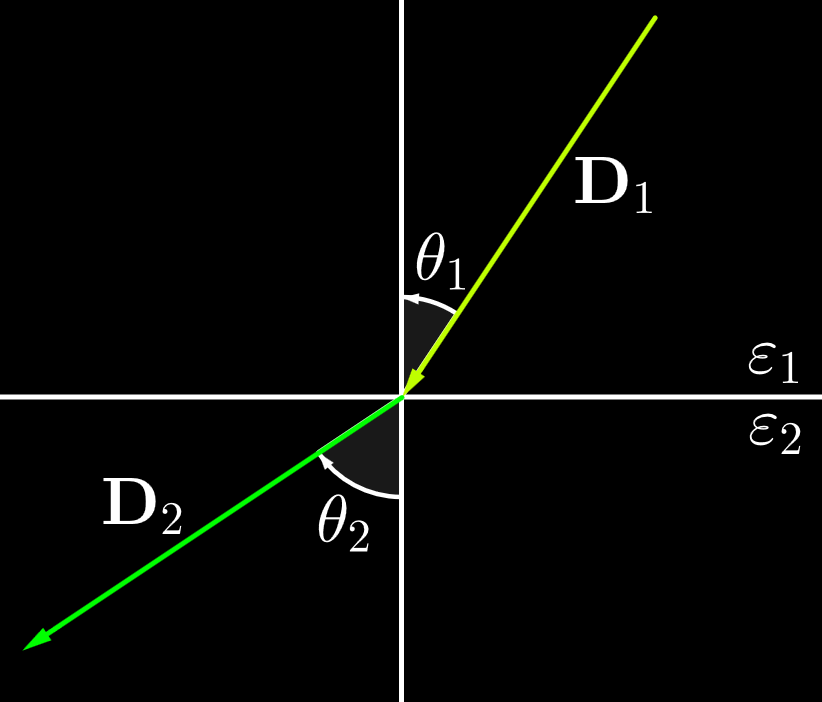
\includegraphics[width=0.7\textwidth]{misc/e-2d.png}
        \caption{The electric displacement field $\vtr{D}_{1}$ diffracts at the boundary between mediums with permittivities $\varepsilon_{1}$ and $\varepsilon_{2}$.
        Beyond the boundary, the field is described by $\vtr{D}_{2}$. The incident angle $\theta_{1}$ and refraction angle $\theta_{2}$ are measured from the surface normal.}
        \label{fig:e2d}
    \end{figure}

    \pagebreak

    The caption can also be placed before the image like in figure \ref{fig:all-waves}.

    \begin{figure}[h!]
        \centering
        \caption{The four most common types of basic digital signals: sine, square, triangle and sawtooth.}
        \label{fig:all-waves}
        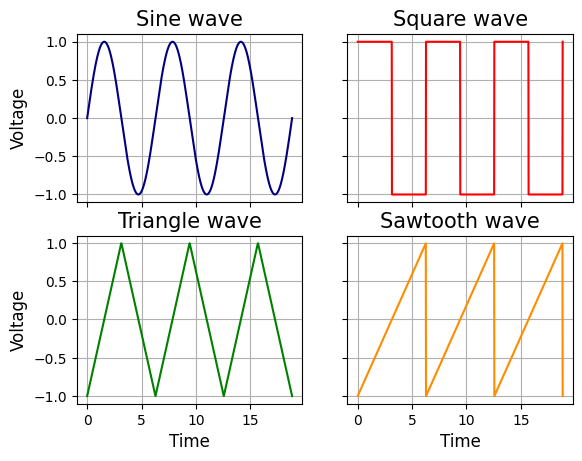
\includegraphics[width=0.9\textwidth]{waves/all-waves.png}
    \end{figure}
    
    \pagebreak

    \section{Multiple Images}

    A figure with two images side by side. Each figure can be referenced independently: figure \ref{fig:mod} contains figures \ref{fig:am} and \ref{fig:fm}.
    This figure utilizes both the graphicx package and the subcaption package.
    
    \begin{figure}[h!]
        \centering
        \caption{Data can be encoded into a transmitted signal using various techniques. Two commonly used techniques are amplitude modulation (AM) and
        frequency modulation (FM).}
        \label{fig:mod}
        \begin{subfigure}{0.4\textwidth}
            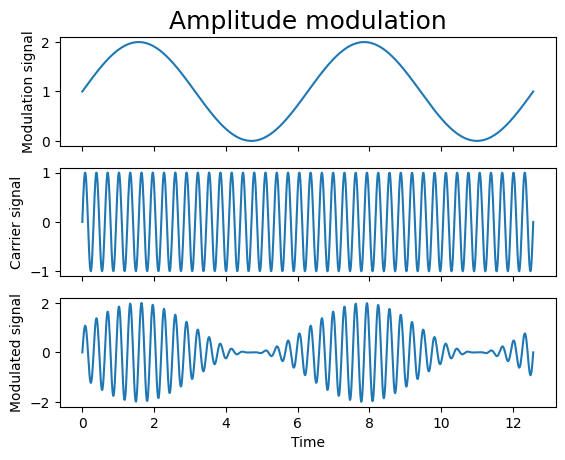
\includegraphics[width=\textwidth]{modulation/amplitude-mod.png}
            \caption{Amplitude modulation varies the amplitude of the carrier signal as a function of the phase of the modulation signal}
            \label{fig:am}
        \end{subfigure}
        \qquad
        \begin{subfigure}{0.4\textwidth}
            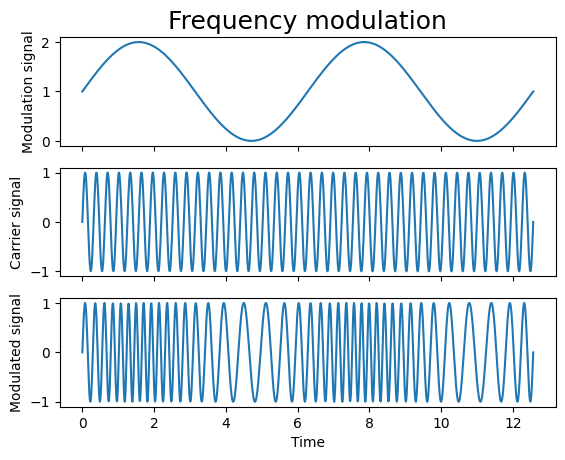
\includegraphics[width=\textwidth]{modulation/frequency-mod.png}
            \caption{Frequency modulation varies the frequency of the carrier signal as a function of the phase of the modulation signal}
            \label{fig:fm}
        \end{subfigure}       
    \end{figure}

    \pagebreak

    A figure with two images on top of each other. Again each figure can be referenced independently: figure \ref{fig:fourier} contains figures \ref{fig:ft} and \ref{fig:ft-log}.
    This figure utilizes both the graphicx package and the subcaption package. The figures' horizontal positions have been changed with the aid of the \texttt{\textbackslash hspace} command.

    \begin{figure}[h!]
        \centering
        \caption{Using the discrete Fourier transform, the frequency spectrum of the noise signal was revealed.}
        \label{fig:fourier}
        \hspace{40pt}\begin{subfigure}{0.6\textwidth}
            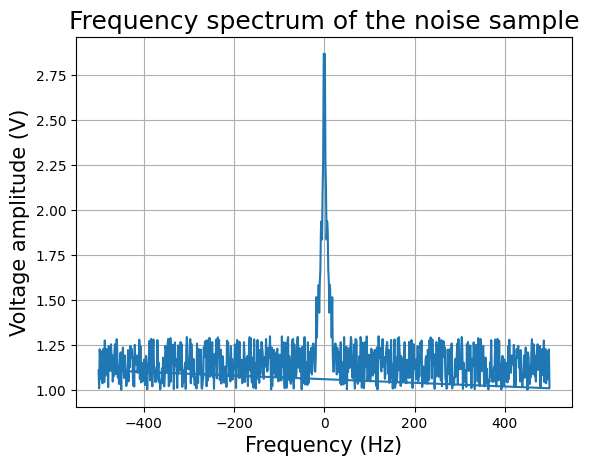
\includegraphics[width=\textwidth]{fourier/fourier.png}
            \caption{A plot of the frequency spectrum shows that the most powerful frequencies in the signal are low frequencies.}
            \label{fig:ft}
        \end{subfigure}
        \newline
        \begin{subfigure}{0.6\textwidth}
            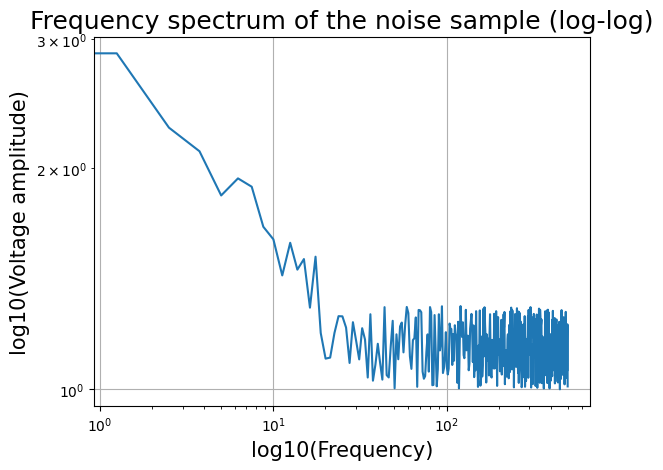
\includegraphics[width=\textwidth]{fourier/fourier-log.png}
            \caption{A log-log plot of the same spectrum reveals that the noise contained in the signal resembles pink noise at lower frequencies and white noise at higher frequencies.}
            \label{fig:ft-log}
        \end{subfigure}   
    \end{figure}

    \pagebreak

    A figure with four images arranged into a square. Again each figure can be referenced independently: figure \ref{fig:waves} contains figures \ref{fig:sine}, \ref{fig:square}, \ref{fig:tri}
    and \ref{fig:saw}. This figure utilizes both the graphicx package and the subcaption package. The subfigures are aligned at the top by passing \texttt{t} as an argument to the subfigure
    environment: \texttt{\textbackslash subfigure[t]\{0.45\textbackslash textwidth\}...}. The horizontal spacing is achieved with the \texttt{\textbackslash hfill} command

    \begin{figure}[h!]
        \centering
        \caption{There are many different types of basic digital signals. The most common types are sine, square, triangle and sawtooth.}
        \label{fig:waves}
        \begin{subfigure}[t]{0.45\textwidth}
            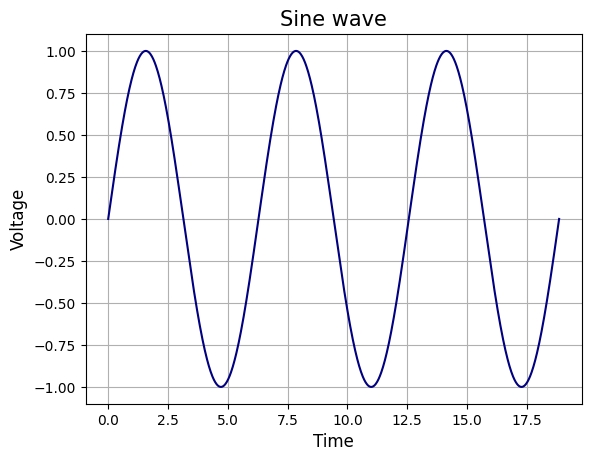
\includegraphics[width=\textwidth]{waves/sine.png}
            \caption{The sine wave is perhaps the most recognizable signal.}
            \label{fig:sine}
        \end{subfigure}
        \hfill
        \begin{subfigure}[t]{0.45\textwidth}
            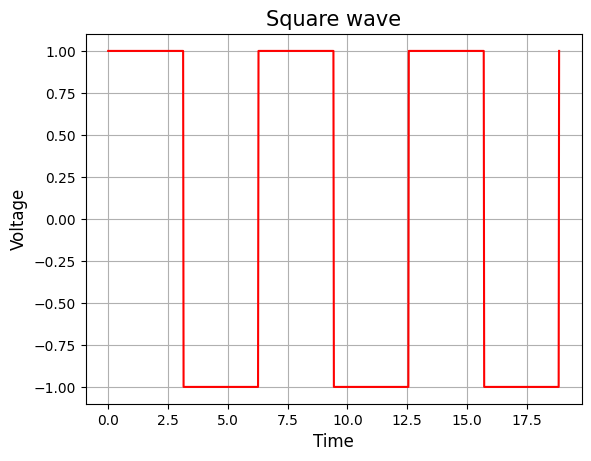
\includegraphics[width=\textwidth]{waves/square.png}
            \caption{The square wave alternates between two extremes.}
            \label{fig:square}
        \end{subfigure}       
        \newline
        \begin{subfigure}[t]{0.45\textwidth}
            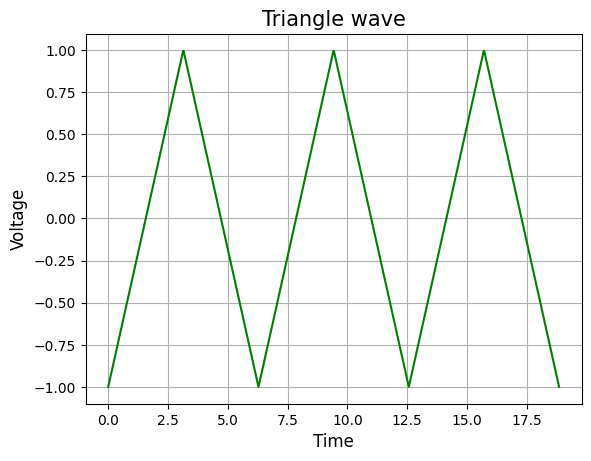
\includegraphics[width=\textwidth]{waves/tri.png}
            \caption{The triangle wave sounds harsh.}
            \label{fig:tri}
        \end{subfigure}
        \hfill
        \begin{subfigure}[t]{0.45\textwidth}
            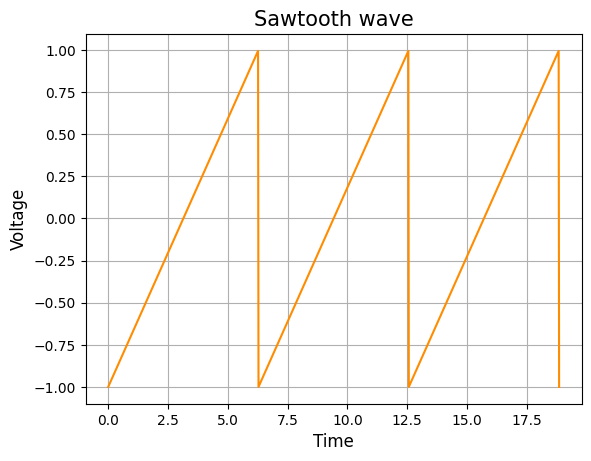
\includegraphics[width=\textwidth]{waves/saw.png}
            \caption{The sawtooth wave is a special case of the triangle wave but common enough to be separately named.}
            \label{fig:saw}
        \end{subfigure}       
    \end{figure}

    \pagebreak

    A figure with 12 images arranged into a rectangle. The subfigures are aligned at the top by passing \texttt{t} as an argument to the subfigure
    environment: \texttt{\textbackslash subfigure[t]\{0.3\textbackslash textwidth\}...}. The horizontal spacing is achieved with the \texttt{\textbackslash hfill} command

    \begin{figure}[h!]
        \centering
        \caption{Different trigonometric and hyperbolic functions plotted on the domain $[-1, 1]$ where each successive picture in a row has a greater power of $x$ in the argument}
        \label{fig:params}
        \begin{subfigure}[t]{0.3\textwidth}
            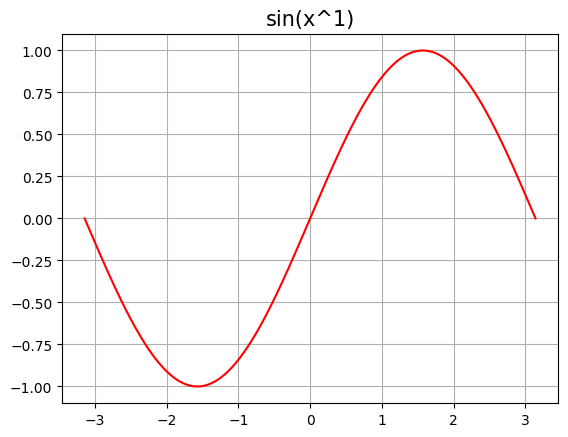
\includegraphics[width=\textwidth]{params/sin-x1.png}
            \caption{Graph of $\sin(x)$}
            \label{fig:sin-x1}
        \end{subfigure}
        \hfill
        \begin{subfigure}[t]{0.3\textwidth}
            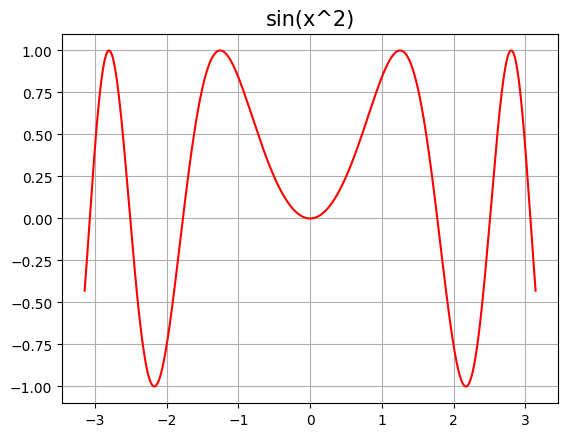
\includegraphics[width=\textwidth]{params/sin-x2.png}
            \caption{Graph of $\sin(x^2)$}
            \label{fig:sin-x2}
        \end{subfigure}       
        \hfill
        \begin{subfigure}[t]{0.3\textwidth}
            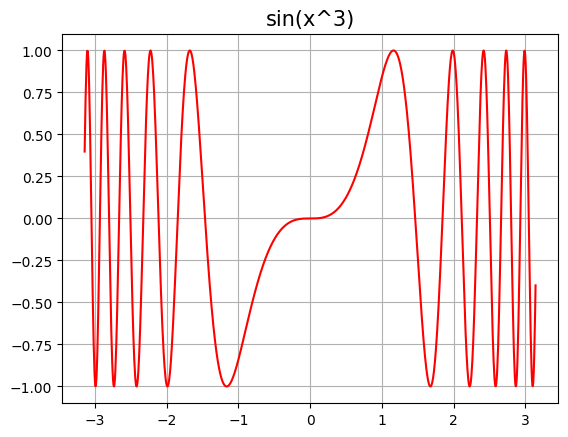
\includegraphics[width=\textwidth]{params/sin-x3.png}
            \caption{Graph of $\sin(x^3)$}
            \label{fig:sin-x3}
        \end{subfigure}
        \newline
        \begin{subfigure}[t]{0.3\textwidth}
            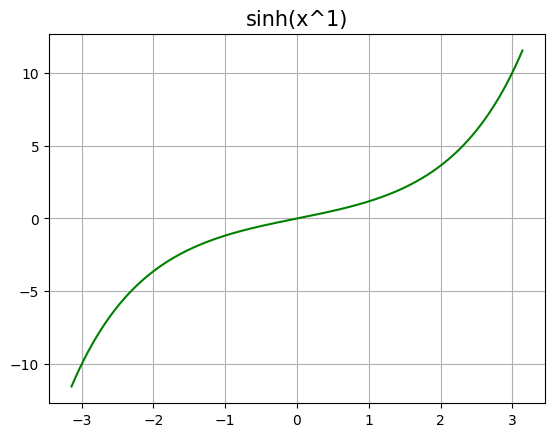
\includegraphics[width=\textwidth]{params/sinh-x1.png}
            \caption{Graph of $\sinh(x)$}
            \label{fig:sinh-x1}
        \end{subfigure}
        \hfill
        \begin{subfigure}[t]{0.3\textwidth}
            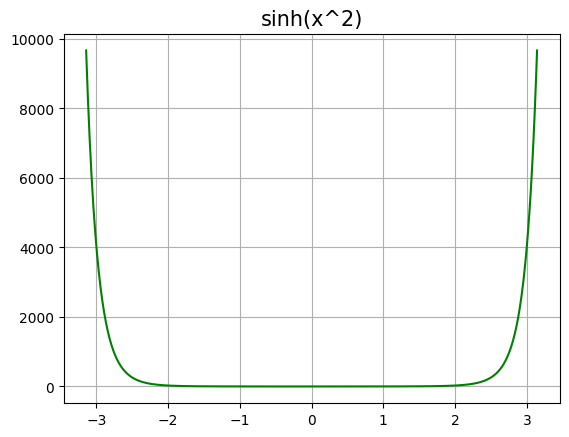
\includegraphics[width=\textwidth]{params/sinh-x2.png}
            \caption{Graph of $\sinh(x^2)$}
            \label{fig:sinh-x2}
        \end{subfigure}       
        \hfill
        \begin{subfigure}[t]{0.3\textwidth}
            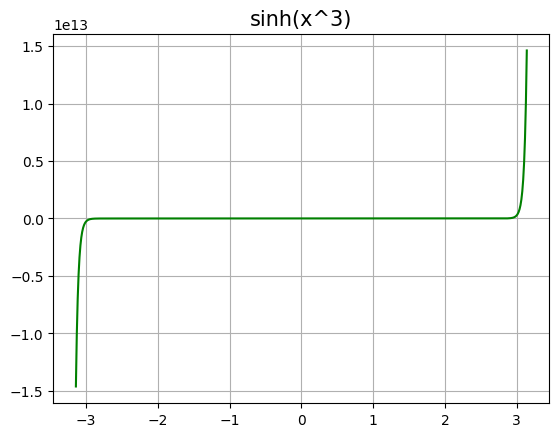
\includegraphics[width=\textwidth]{params/sinh-x3.png}
            \caption{Graph of $\sinh(x^3)$}
            \label{fig:sinh-x3}
        \end{subfigure}
        \newline
        \begin{subfigure}[t]{0.3\textwidth}
            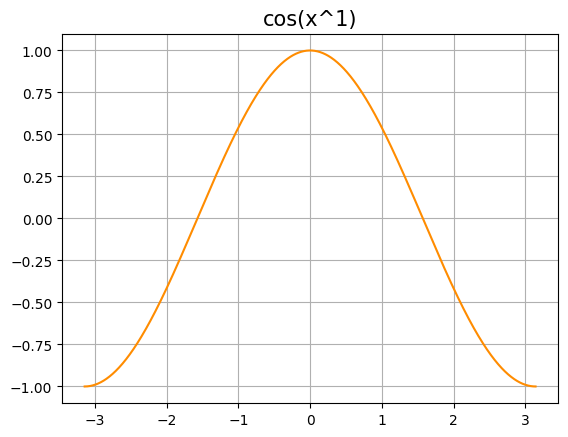
\includegraphics[width=\textwidth]{params/cos-x1.png}
            \caption{Graph of $\cos(x)$}
            \label{fig:cos-x1}
        \end{subfigure}
        \hfill
        \begin{subfigure}[t]{0.3\textwidth}
            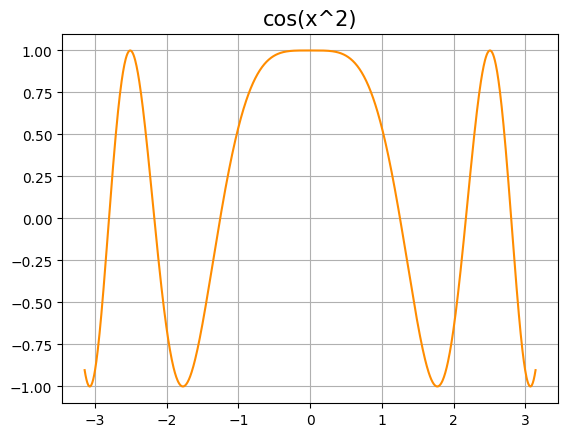
\includegraphics[width=\textwidth]{params/cos-x2.png}
            \caption{Graph of $\cos(x^2)$}
            \label{fig:cos-x2}
        \end{subfigure}       
        \hfill
        \begin{subfigure}[t]{0.3\textwidth}
            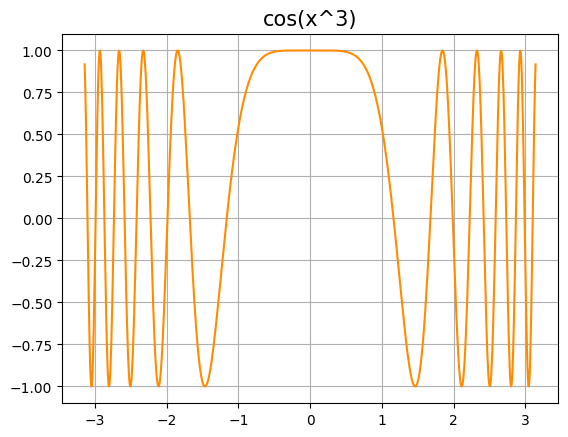
\includegraphics[width=\textwidth]{params/cos-x3.png}
            \caption{Graph of $\cos(x^3)$}
            \label{fig:cos-x3}
        \end{subfigure}
        \newline
        \begin{subfigure}[t]{0.3\textwidth}
            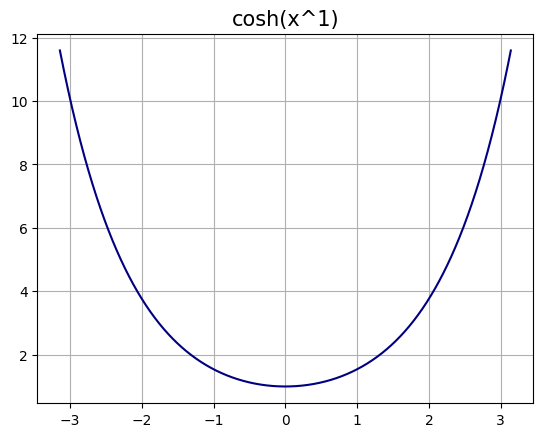
\includegraphics[width=\textwidth]{params/cosh-x1.png}
            \caption{Graph of $\cosh(x)$}
            \label{fig:cosh-x1}
        \end{subfigure}
        \hfill
        \begin{subfigure}[t]{0.3\textwidth}
            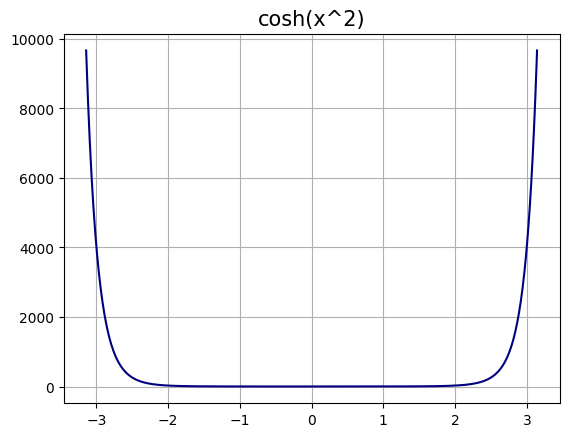
\includegraphics[width=\textwidth]{params/cosh-x2.png}
            \caption{Graph of $\cosh(x^2)$}
            \label{fig:cosh-x2}
        \end{subfigure}       
        \hfill
        \begin{subfigure}[t]{0.3\textwidth}
            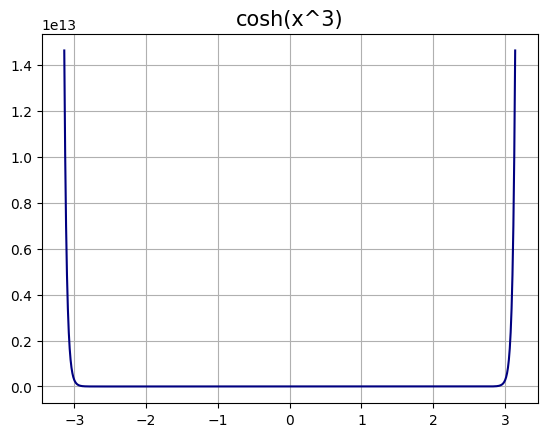
\includegraphics[width=\textwidth]{params/cosh-x3.png}
            \caption{Graph of $\cosh(x^3)$}
            \label{fig:cosh-x3}
        \end{subfigure}
    \end{figure}

    

\end{document}
